\chapter{Wstęp}

\section{Wprowadzenie}

W ostatnich kilkudziesięciu latach ilość informacji, z~jaką styka się człowiek w~ciągu swojego życia, wzrosła wielokrotnie. Zjawisko to nie miało miejsca nigdy wcześniej w~historii ludzkości. W~związku w~wszechobecnością wszelkiego typu treści ludzie wypracowali sobie odruchy podświadomego filtrowania informacji, które z~ich punktu widzenia są niepotrzebne lub nieinteresujące. Stawia to przed twórcami zajmującymi się wizualizacją nowe wyzwania polegające na zwróceniu uwagi potencjalnego odbiorcy i~prezentacji informacji w~szybki, prosty i~atrakcyjny sposób. Ma to szczególne znaczenie w~wymiarze komercyjnym, gdzie od skuteczności reklamy w~dużej mierze zależy powodzenie przedsiębiorstwa.

Tablice informacyjne i~reklamowe oparte o~wyświetlacze LED są zauważalne z~powodu dobrej widoczności zarówno w~dzień, jak i~w~nocy oraz prezentacji obrazów ruchomych, co naturalnie przyciąga wzrok odbiorcy.

Zapoznając się z~istniejącymi urządzeniami tego typu zauważa się archaiczność stosowanych w~nich rozwiązań technicznych, takich jak użycie interfejsów szeregowych w~standardzie RS232 i~braku łatwych w~obsłudze programów do tworzenia animacji. Często producenci nie udostępniają takiego programu użytkownikom, oferując w~zamian usługę tworzenia animacji, co generuje dodatkowe koszty dla właściciela urządzenia.

Opracowano więc projekt tablicy świetlnej, która posiada złącze USB do komunikacji z~komputerem PC oraz przechowuje dane na powszechnie stosowanej karcie pamięci typu SD.~Urządzenie, widoczne na rysunku \ref{zdj-calosc}, ma budowę modułową, co przy pewnych modyfikacjach oprogramowania umożliwia zmianę rozmiaru tablicy z~domyślnych ośmiu paneli do mniejszej ich liczby lub też ustawienie w~dwa rzędy (konfiguracja $4 \times 2$).

\begin{figure}[htb]
	\begin{center}
		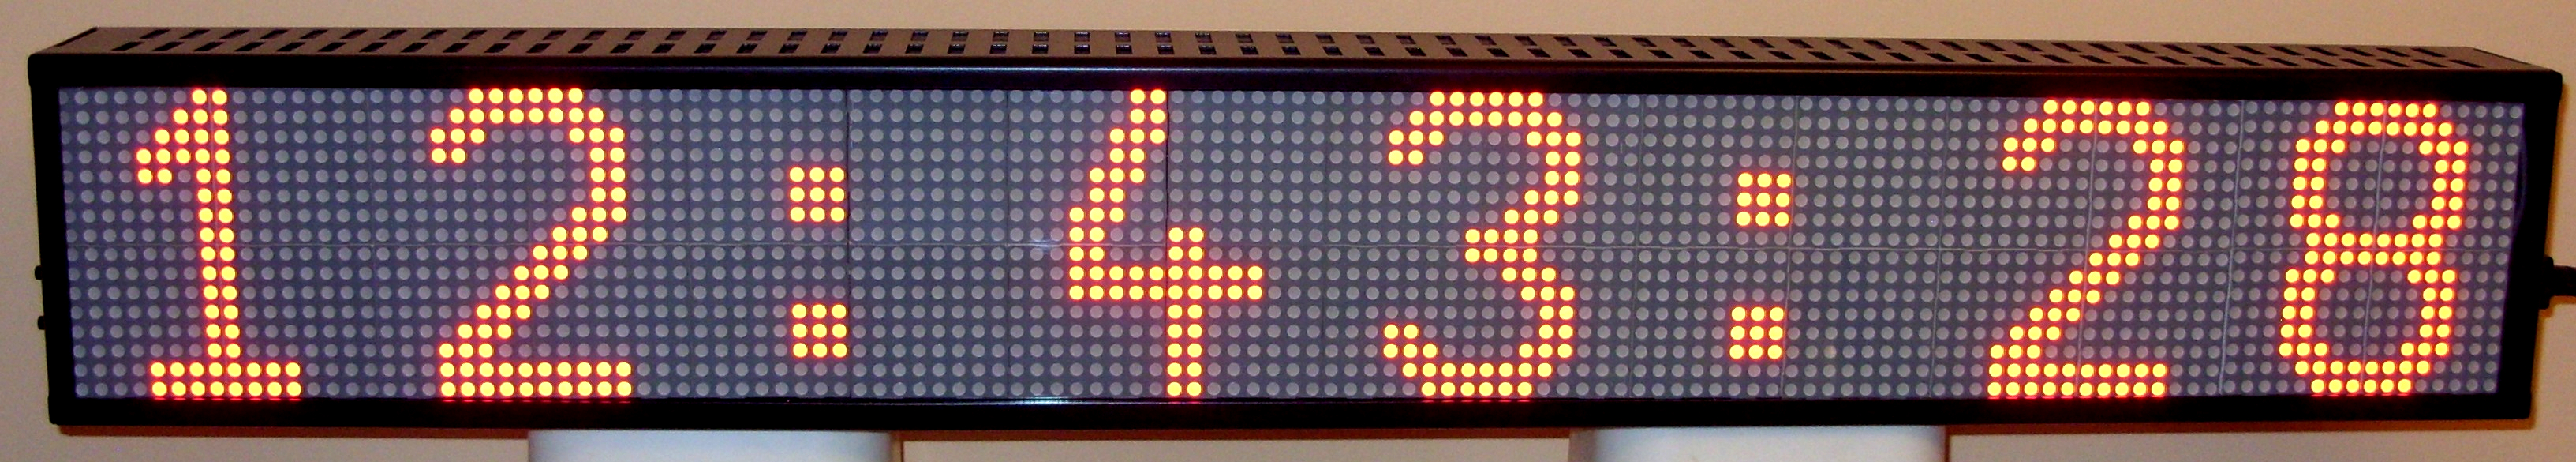
\includegraphics[width=\textwidth]{figures/overall.jpg}
	\end{center}
	\caption{Widok ogólny urządzenia.}
	\label{zdj-calosc}
\end{figure}

Celem pracy jest zaprojektowanie i~wykonanie sterownika diodowej matrycy świetlnej wraz z~oprogramowaniem dla komputera PC umożliwiającym tworzenie animacji tekstowych i~graficznych możliwych do wyświetlenia na skonstruowanym urządzeniu.

\section{Struktura pracy}

Niniejsza praca składa się pięciu rozdziałów oraz dodatku. Rozdział \textit{Podstawy teoretyczne} omawia w~ogólny sposób najważniejsze zagadnienia związane z~projektem, jak idea wyświetlania multipleksowego na matrycach LED, opis mikrokontrolera AT90USB647, interfejsu USB i~kart pamięci SD oraz podstawowe informacje na temat fontów komputerowych.

Rozdział trzeci zawiera zarys projektu systemu oraz opis formatów plików służących do wymiany informacji między urządzeniem a~komputerem. Rozdział czwarty szczegółowo opisuje wykonanie systemu na trzech obszarach: urządzenia elektronicznego, oprogramowania mikrokontrolera oraz programu na komputer PC.~Rozdział piąty stanowi podsumowanie pracy.  W~dodatkach zamieszczono: instrukcje obsługi dla użytkowników omawiające sposób nawigacji po menu tablicy i~tworzenie animacji w~programie komputerowym, parametry zasilacza sieciowego oraz spis zawartości dołączonej płyty CD.

Niniejszą pracę realizowało trzech niżej wymienionych autorów. Sekcje poświęcone danemu zagadnieniu są autorstwa osoby, która zajmowała się nim przy projektowaniu i~wykonywaniu urządzenia. Poniżej przedstawiono podział zadań.

\textbf{Mikołaj Błajek} opracował obsługiwany przez urządzenie format plików M2F oraz zaimplementował jego odtwarzanie na komputerze PC oraz na sterowniku. Zaimplementował takie elementy funkcjonalności tablicy, jak menu, zegar wraz z~jego ustawianiem oraz wybór i~wczytywanie plików animacji. Zaprojektował dwa fonty, dostosowując je do określonych wymagań.~Poza tym wykonał drobne prace montażowe.

\textbf{Filip Rachwalak} opracował format plików MMF, zaprojektował i~zaimplementował aplikację do tworzenia animacji na komputerze PC, w~szczególności, zaprojektował metody rysowania wewnątrz obszarów (\textit{obszar} --- patrz \ref{slownik}) jak i~samych obszarów i~dodawania efektów tekstowych. Zaimplementował również generator plików wyjściowych animacji. Dokonał montażu całego urządzenia z~dostarczonych płytek drukowanych i~elementów elektronicznych.

\textbf{Michał Słomkowski} w~ramach niniejszej pracy zaprojektował urządzenie od strony sprzętowej, w~szczególności: opracował schemat ideowy modułu sterownika wraz z~projektem ścieżek płytki drukowanej oraz zaprogramował elementy oprogramowania mikrokontrolera na niskim poziomie abstrakcji, jak obsługa przerwań, portów wejścia-wyjścia, czasomierzy, zintegrował używane biblioteki obsługi kart SD, magistrali USB oraz systemu plików FAT.~Dokonał również montażu sterownika.

\section{Słownik pojęć}
\label{slownik}

W celu uniknięcia niejednoznaczności podczas czytania niniejszej pracy, poniżej opisano stosowane w~niej terminy.

\begin{itemize}
	\item \textit{Animacja} --- pełna sekwencja klatek (\textit{klatka} --- patrz niżej) odtwarzana przez mikrokontroler na tablicy. Jest wizualizacją wygenerowanego przez aplikację pliku,

	\item \textit{driver} --- płytka drukowana, na której znajdują się wzmacniacze mocy sterujące wyświetlaczami,

	\item \textit{efekt} --- pojedyncza czynność modyfikująca tekst lub grafikę w~obrębie \textit{obszaru} np. \textit{Przewijanie w~lewo}, wyrównanie tekstu \textit{Do środka} lub \textit{Negatyw},
	
	\item \textit{font} --- zestaw znaków drukarskich o~wspólnych cechach \cite{fonts},

	\item \textit{ekran} --- odwzorowanie powierzchni tablicy w~graficznym interfejsie użytkownika, widoczne w~jego głównej części. Wymiary ekranu odpowiadają faktycznym wymiarom tablicy ($128 \times 16$ elementów świecących),
	
	\item \textit{font} --- oznaczają zestaw znaków pisarskich, opisujących kształt i wielkość liter, czcionka,
	
	\item \textit{klatka} --- pojedynczy stan ekranu. Animacja składa się z~następujących po sobie klatek,

	\item \textit{magistrala} --- zestaw szyn i~linii sygnałowych pomiędzy sterownikiem a~drajwerem, znajdujących się na płytce drukowanej magistrali,

	\item \textit{matryca} --- płytka drukowana grupująca cztery wyświetlacze $8 \times 8 $ w~jeden o~wymiarach $16 \times 16$. Jest połączona z~płytką drajwera,

	\item \textit{obszar} --- powierzchnia w~kształcie prostokąta rysowana przez użytkownika na ekranie za pomocą myszki. Użytkownik definiuje wyświetlaną treść w~obrębie zaznaczonej powierzchni,

	\item \textit{piksel} --- pojedyncza ,,dioda'' tablicy i~jej odwzorowanie na ekranie w~postaci białego pojedynczego kwadratu,

	\item \textit{plik animacji} --- plik o~rozszerzeniu \texttt{.m2f} wygenerowany przez aplikację, który zawiera pełną animację,

	\item \textit{projekt} --- 1. efekt pracy użytkownika: rozmieszczone na ekranie i~wyspecyfikowane obszary. Projekt można zapisać jako plik z~rozszerzeniem \texttt{.mmf} i~otworzyć go później. 2. całokształt pracy wykonanej przez autorów,

	\item \textit{sterownik} --- płytka drukowana zawierająca mikrokontroler AVR, sterująca zestawami,

	\item \textit{tablica} --- całe urządzenie, wszystkie moduły połączone w~całość,

	\item \textit{typografia} --- dziedzina wiedzy o zasadach składu drukarskiego, sposób prezentacji tekstu w sposób czytelny i estetyczny \cite{fonts},

	\item \textit{zestaw} --- połączone ze sobą płytki: matrycy, drajwera i~magistrali.
\end{itemize}
